\documentclass[12pt]{article}

\setlength\parindent{0pt}
\newcommand{\myt}[1]{\textbf{\underline{#1}}}

\usepackage{mathtools}
\usepackage{amssymb}
\usepackage{graphicx}

\title{\vspace{-15ex}Math 239 Lecture 25\vspace{-1ex}}
\date{July 8th, 2015}
\author{Graham Cooper}

\begin{document}
	\maketitle
	Items:\\
	\begin{itemize}
		\item Planar Graphs
		\item Euler's Formula
	\end{itemize}
	
	\section*{Planar Graphs}
	\subsection*{Definitions}
	\myt{Definition:} A \underline{planar embedding} of a graph G is adrawing on a plane such that vertices are at different points and edges do not cross each other. A graph that has a planar embedding is called a \underline{planar graph}\\
	
	Example:\\
	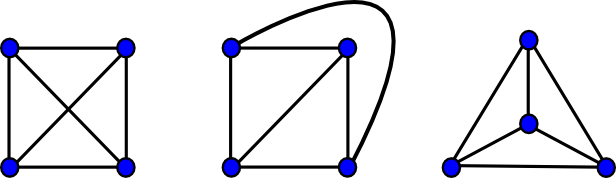
\includegraphics[scale=0.5]{planar.png}\\
	The first graph is NOT planar, the other two are.\\
	
	\myt{Definition} A \underline{face} of a planar embedding is a connected region on the plane. Two faces are \underline{adjacent} if they share at least one edge\\
	
	Example:\\
	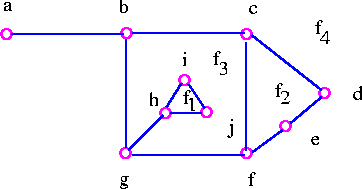
\includegraphics[scale=0.5]{faces.png}\\
	F4 is the outer face, the unbounded face\\
	
	\myt{Definition:} For a connected graph, the \underline{boundary walk} of a face is a cloased walk using the edges around teh boundary.\\
	
	Example:\\
	f3: \{b,c,f,g,b\}\\
	f1: \{i,j,h,i\}\\
	
	\myt{Definition:} The \underline{degree} of a face deg(f) is the length of its boundary walk\\
	
	\subsection*{Theorems}
	\myt{Handshaking Lemma for faces:} Let G be a plannar graph with a planar embedding wehre F is the set of all faces. Then\\
	$$\sum_{f \in F} deg(f) = 2|E(G)|$$
	\myt{Proof}: Each edge contrubutes 2 to the sume of degrees, 1 for each side of the edge.\\
	
	A bridge has the same face on both sides. A non-bridge has different faces on each side.\\
	
	\myt{Jordan curve theorem:} Every simple closed curve on the plan seperates the plane into 2 parts, one inside, one outside\\
	
	This is not true on the surface of a torus\\
	
	G is connected and plannar. G has only 1 face if and only if G is a tree. (no cycles). IF G has at least 2 faces, then each face must be seperated from other faces via a cycle on its boundary $\implies$ degree of each face is at least 3 contains a cycle
	
	
\end{document}
